% !TEX root = thesis-ex.tex
Quantum Chromodynamics is a gauge theory with SU(3) symmetry that describes the dynamics of the strong interactions between quarks and gluons.
It is part of the Standard Model \cite{Gaillard:1998ui}, the building blocks of which are shown in Figure~\ref{fig:sm_particles}.

%The Standard Model (SM) \cite{Gaillard:1998ui} describes the interactions between elementary particles that are listed in Figure~\ref{fig:sm_particles}.It is one the most successful theories in physics and describes three of the four fundamental forces of nature.These are the strong interaction, the weak interaction, and the electromagnetic interaction.A quantum theory for gravity is not part of the SM.

\begin{figure}[htbp]
\begin{center}
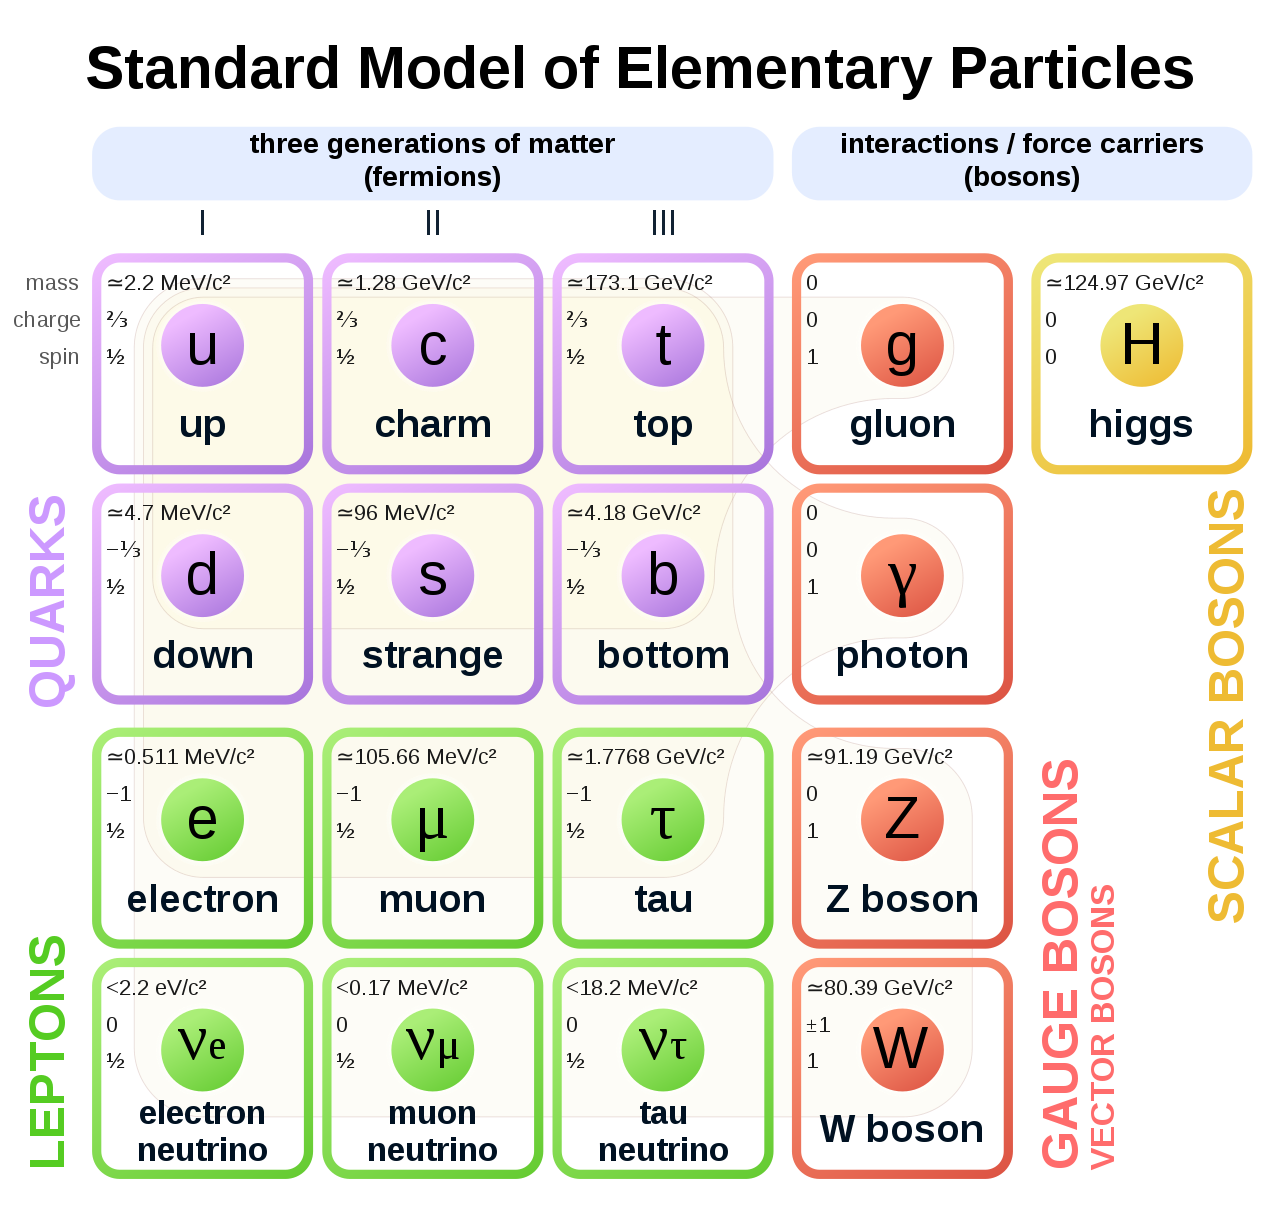
\includegraphics[width=0.5\textwidth]{figures/theory/SM}
\caption{The elementary particles of the standard model.
Figure from Ref.~\cite{SMpict}.}
\label{fig:sm_particles}
\end{center}
\end{figure}

%Within the SM, the dynamics of the strong interactions involving quarks and gluons are described by Quantum Chromodynamics (QCD), 

Quarks are fermions with a spin of $1/2$, and carry a fractional electric charge as well as a color charge.
They all have mass and come in six flavors: up, down, strange, charm, top, bottom.
The lightest quarks (u and d) combine and form stable particles, while the heavier quarks can only be produced in energetic environments and decay rapidly.
Gluons are gauge bosons (force carriers) with a spin of $1$, and are what hold quarks together.
The dynamics of the quarks and gluons, collectively referred to as partons, are described by the QCD Lagrangian given by \cite{Beringer:1481544}:

\begin{align}
\mathcal{{L}}_{\mathrm{QCD}} = \sum_q \bar{\psi}_{q,a} (i \gamma^\mu \partial_\mu \delta_{ab} - g_s \gamma^\mu t_{ab}^C \mathcal{A}_\mu^C - m_q \delta_{ab}) \psi_{q,b} - \frac{1}{4} F_{\mu\nu}^A F^{A \mu\nu}
\end{align}
where $\psi_{q,a}$ and $\psi_{q,b}$ are quark-field spinors for a quarks with flavor $q$, mass $m_q$, and color $a$ and $b$ respectively, with the values for $a$ and $b$ ranging  from 1 to 3 (for the three colors).
The $\mathcal{A_\mu^C}$ corresponds to the gluon field with $C$ taking values from 1 through 8 (for the 8 types of gluons).
The $t_{ab}^C$ corresponds to the Gell-Mann matrices that are the generators of the SU(3) group, and dictate the rotation of the quarks color in SU(3) space when it interacts with a gluon.
The coupling constant is encoded within $g_s$, which is defined by $g_s \equiv \sqrt{4 \pi \alpha_s}$.
The field tensor $F_{\mu\nu}^A$ can be written in terms of the structure constants of the SU(3) group $f_{ABC}$, and is given by:

\begin{align}
F_{\mu\nu}^A = \partial_\mu \mathcal{A}_\nu^A - \partial_\nu \mathcal{A}_\mu^A - g_s f_{ABC} \mathcal{A}^B \mathcal{A}^C
\end{align}
While many parallels can be drawn between Quantum Electrodynamics (QED, the theory that describes photons and electrons) and QCD, the main difference between the two comes from the gluon-gluon interactions allowed in QCD, making it non-Abelian.
These interactions can be summarized as shown in Figure~\ref{fig:qcd_diagrams}.

\begin{figure}[htbp]
\begin{center}
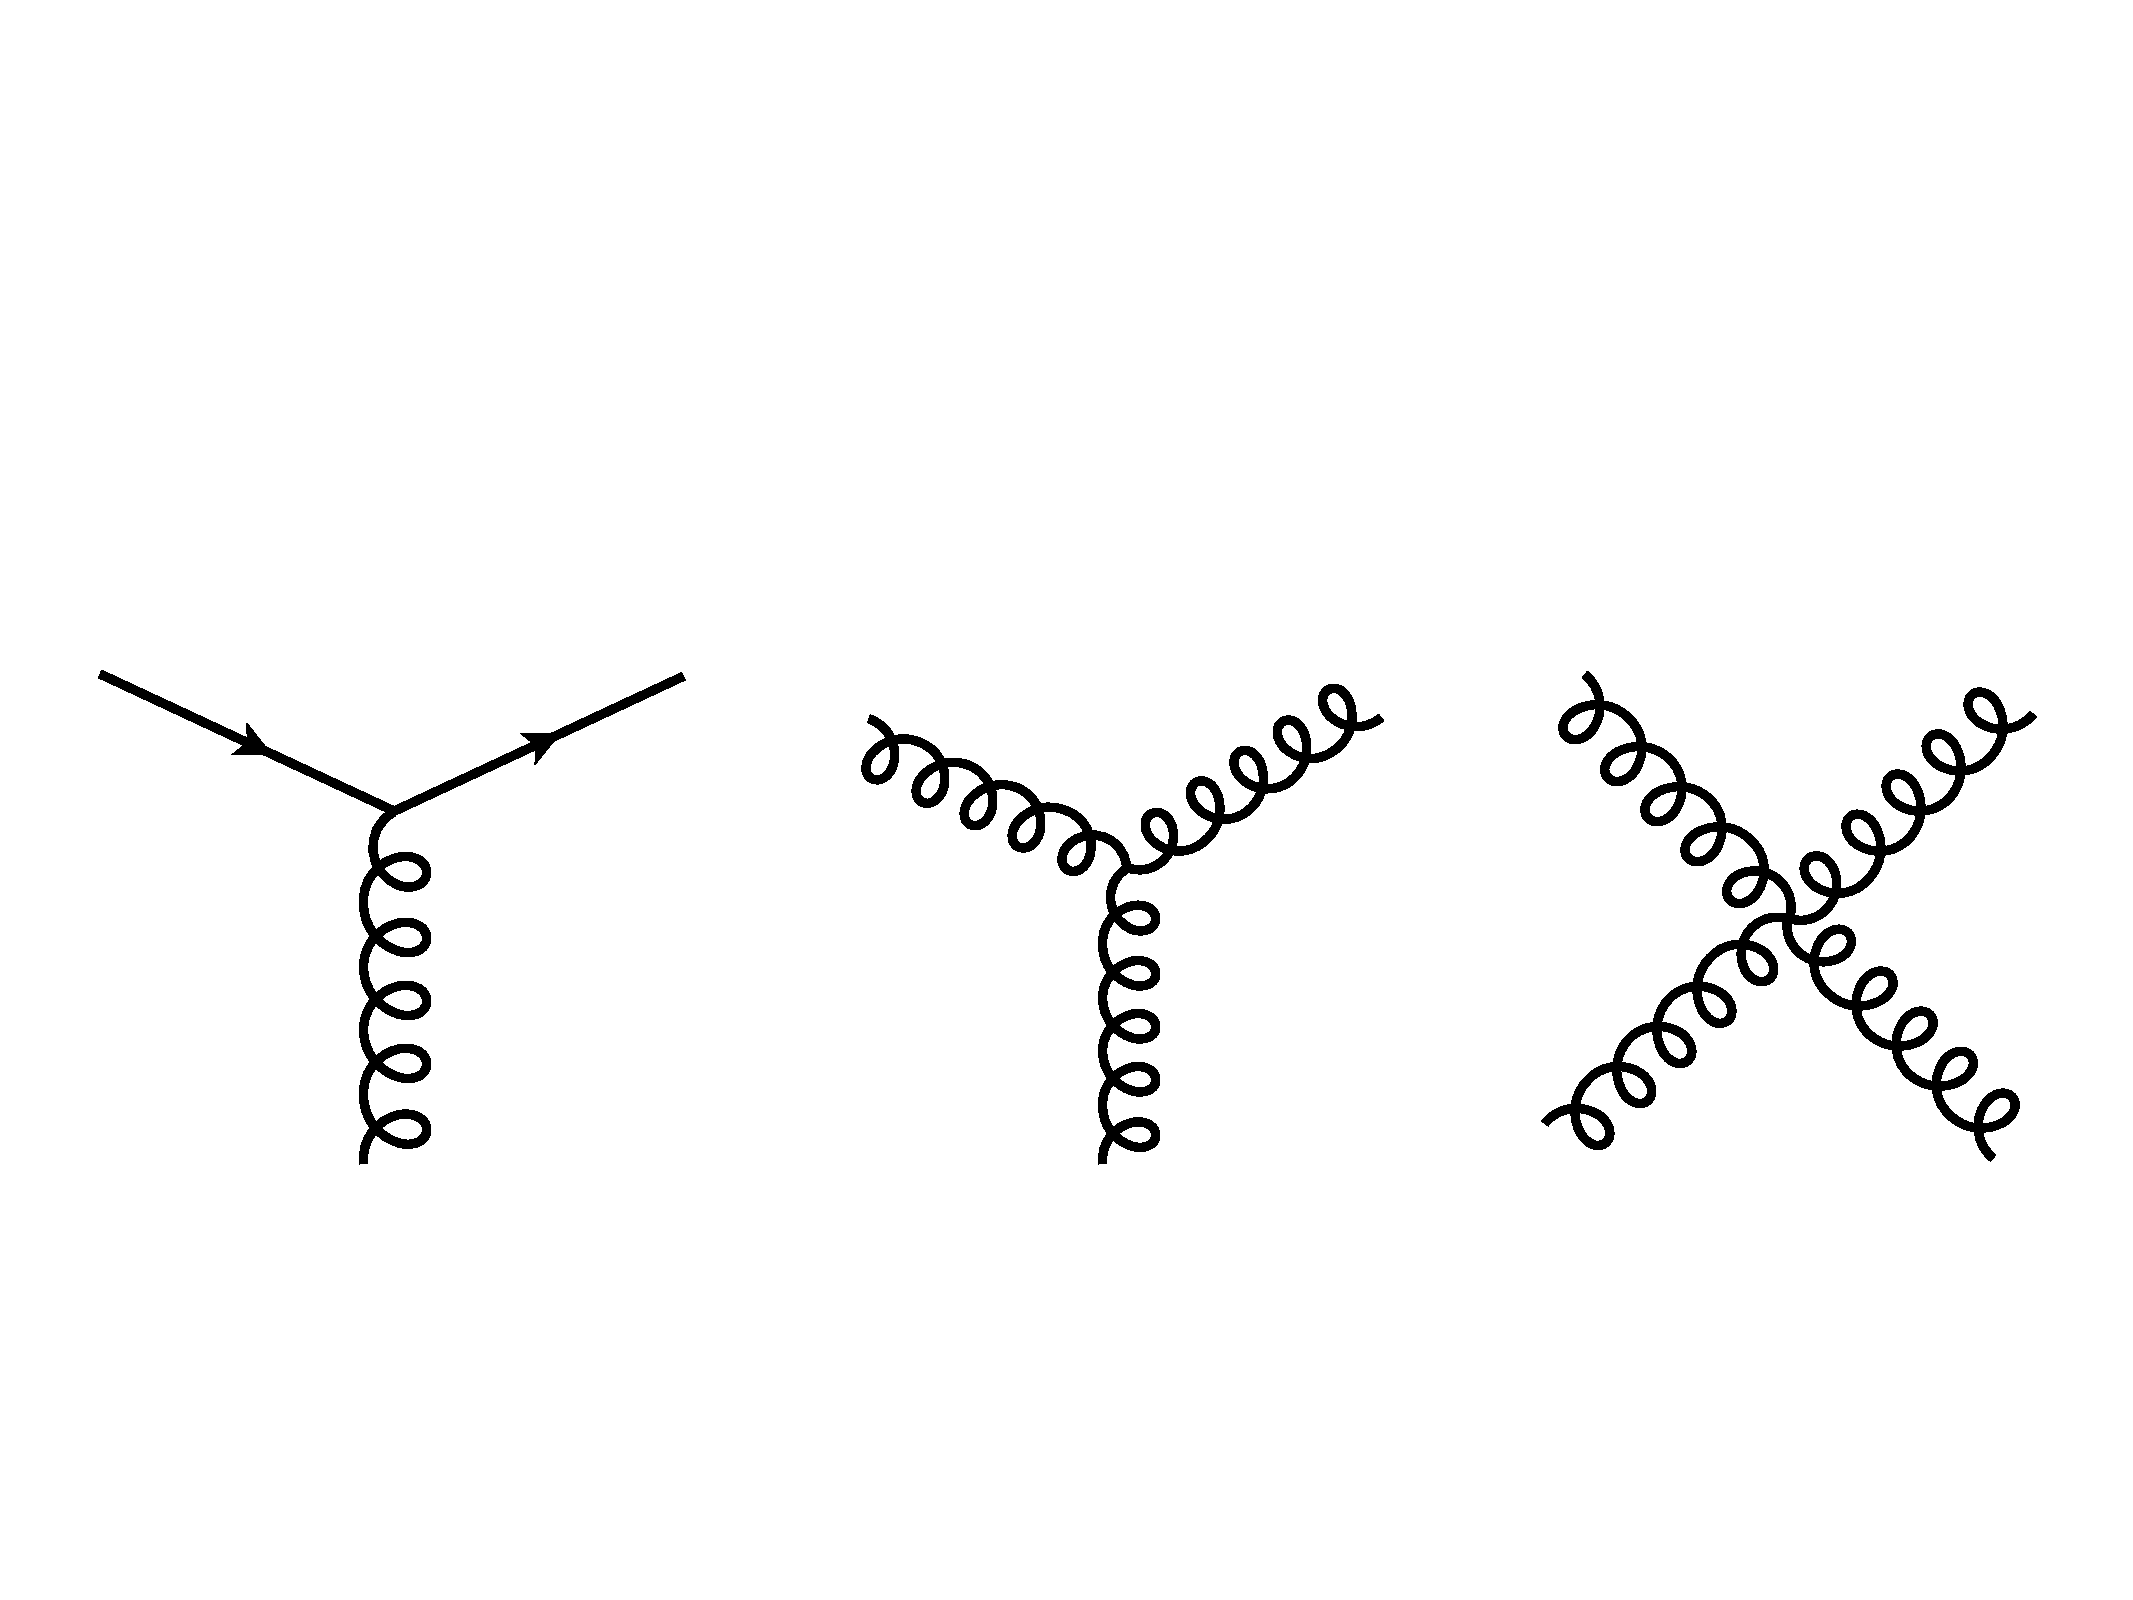
\includegraphics[width=0.6\textwidth]{figures/theory/qcd_diagrams}
\caption{The allowed vertices in QCD.
The vertices involving three or four gluons are unique to QCD and do not have a QED analog.}
\label{fig:qcd_diagrams}
\end{center}
\end{figure}

A core feature of QCD is that the coupling constant \alphas\ has an energy dependence shown in Figure~\ref{fig:running_coupling}.
This dependence can be expressed in terms of the $\beta$ function as

\begin{align}
Q^2 \frac{\partial \alpha_s (Q^2)}{\partial Q^2} = \beta(\alpha_s (Q^2))
\end{align}
where $Q$ is the momentum transfer in the particle reaction
\footnote{The momentum transfer $Q$ is the amount of momentum transferred in a scattering process.}.
The beta function can be expressed using perturbative QCD (pQCD) as:

\begin{align}
\beta( \alpha_s ) = - (b_0 \alpha_s^2 + b_1 \alpha_s^3 + b_2 \alpha_s^4...)
\end{align}
where the coefficients $b_i$ depend on the number of colors and flavors.
This running coupling constant is small and asymptotically tends to zero at large energy scales (or at small distances) and is large at small energy scales (large distances).
This running coupling phenomenon leads to two key behaviors: asymptotic freedom and color confinement.

\begin{figure}[htbp]
\begin{center}
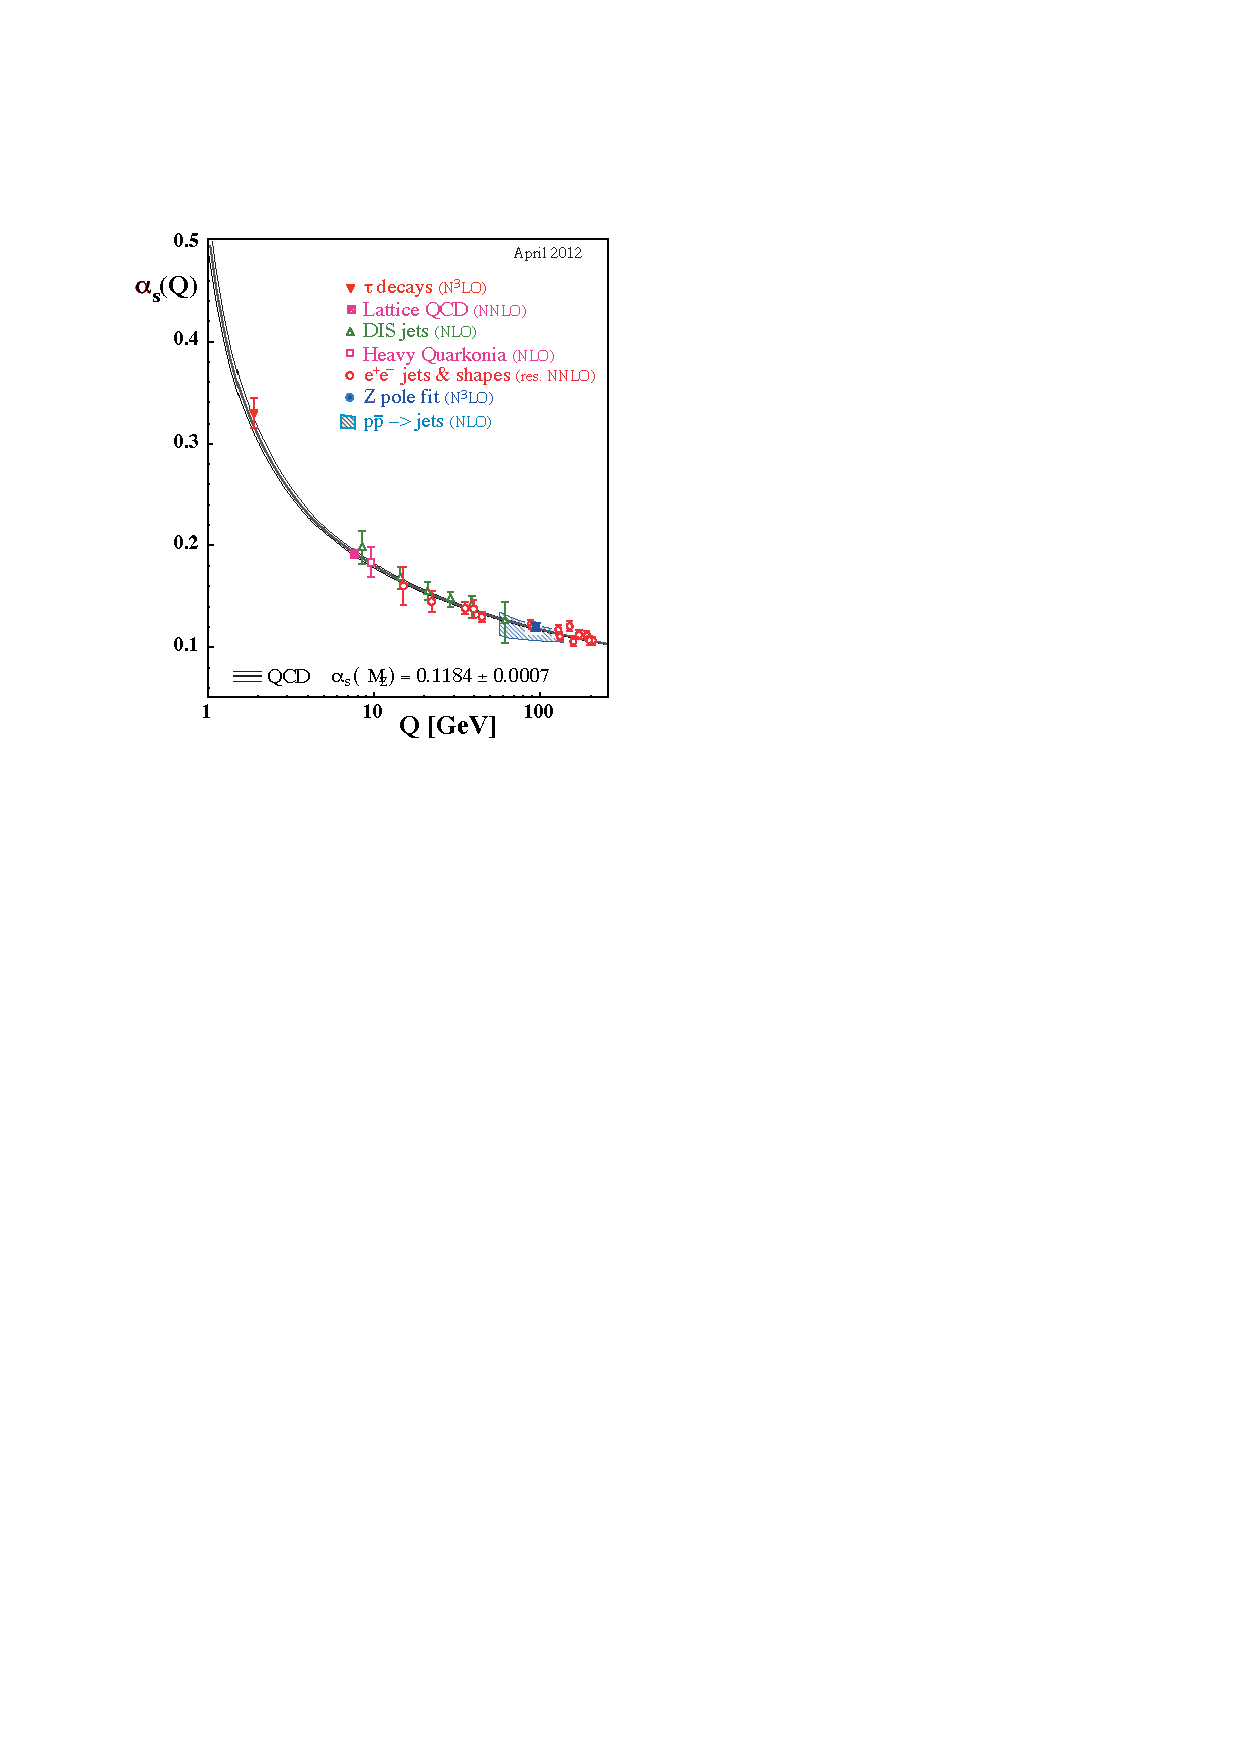
\includegraphics[width=0.5\textwidth]{figures/theory/running_coupling}
\caption{The running coupling constant $\alpha_s$ as a function of the momentum transfer $Q$.
Figure from Ref.~\cite{Beringer:1481544}.}
\label{fig:running_coupling}
\end{center}
\end{figure}



\subparagraph{Asymptotic Freedom: }
At high energy scales (small distances), the QCD coupling constant $\alpha_s$ is small and tends to zero, implying a free particle behavior of quarks and gluons \cite{PhysRevLett.30.1343, PhysRevD.8.3633}.
This has been observed by a variety of deep inelastic scattering (DIS) experiments \cite{Deur:2014vea, Kim:1998kia, Altarelli:1996nm, RevModPhys.63.597, Kataev:2001kk, Alekhin:2012ig, Alekhin:2013nua, Blumlein:2006be, Aaron:2007xx, Chekanov:2007pa, Chekanov:2008af, Abramowicz:2010cka, Abramowicz:2010ke, Aaron:2009vs}.
These scattering experiments shown in Figure~\ref{fig:dis_schematic}, probe the interior of a nucleon using highly energetic leptons like electrons.
The electron scatters off of the target proton, producing a lepton and a hadron shower.
First done by MIT-SLAC \cite{PhysRevLett.23.930, PhysRevLett.23.935}, these DIS experiments showed the weak $Q^2$ dependence on the inelastic scattering cross-sections, as well as Bjorken scaling \cite{PhysRev.179.1547}, where the proton structure functions are independent of the momentum transfer.
These experiments revealed the point-like constituents of the proton and paved the road to an asymptotically free theory.

\begin{figure}[htbp]
\begin{center}
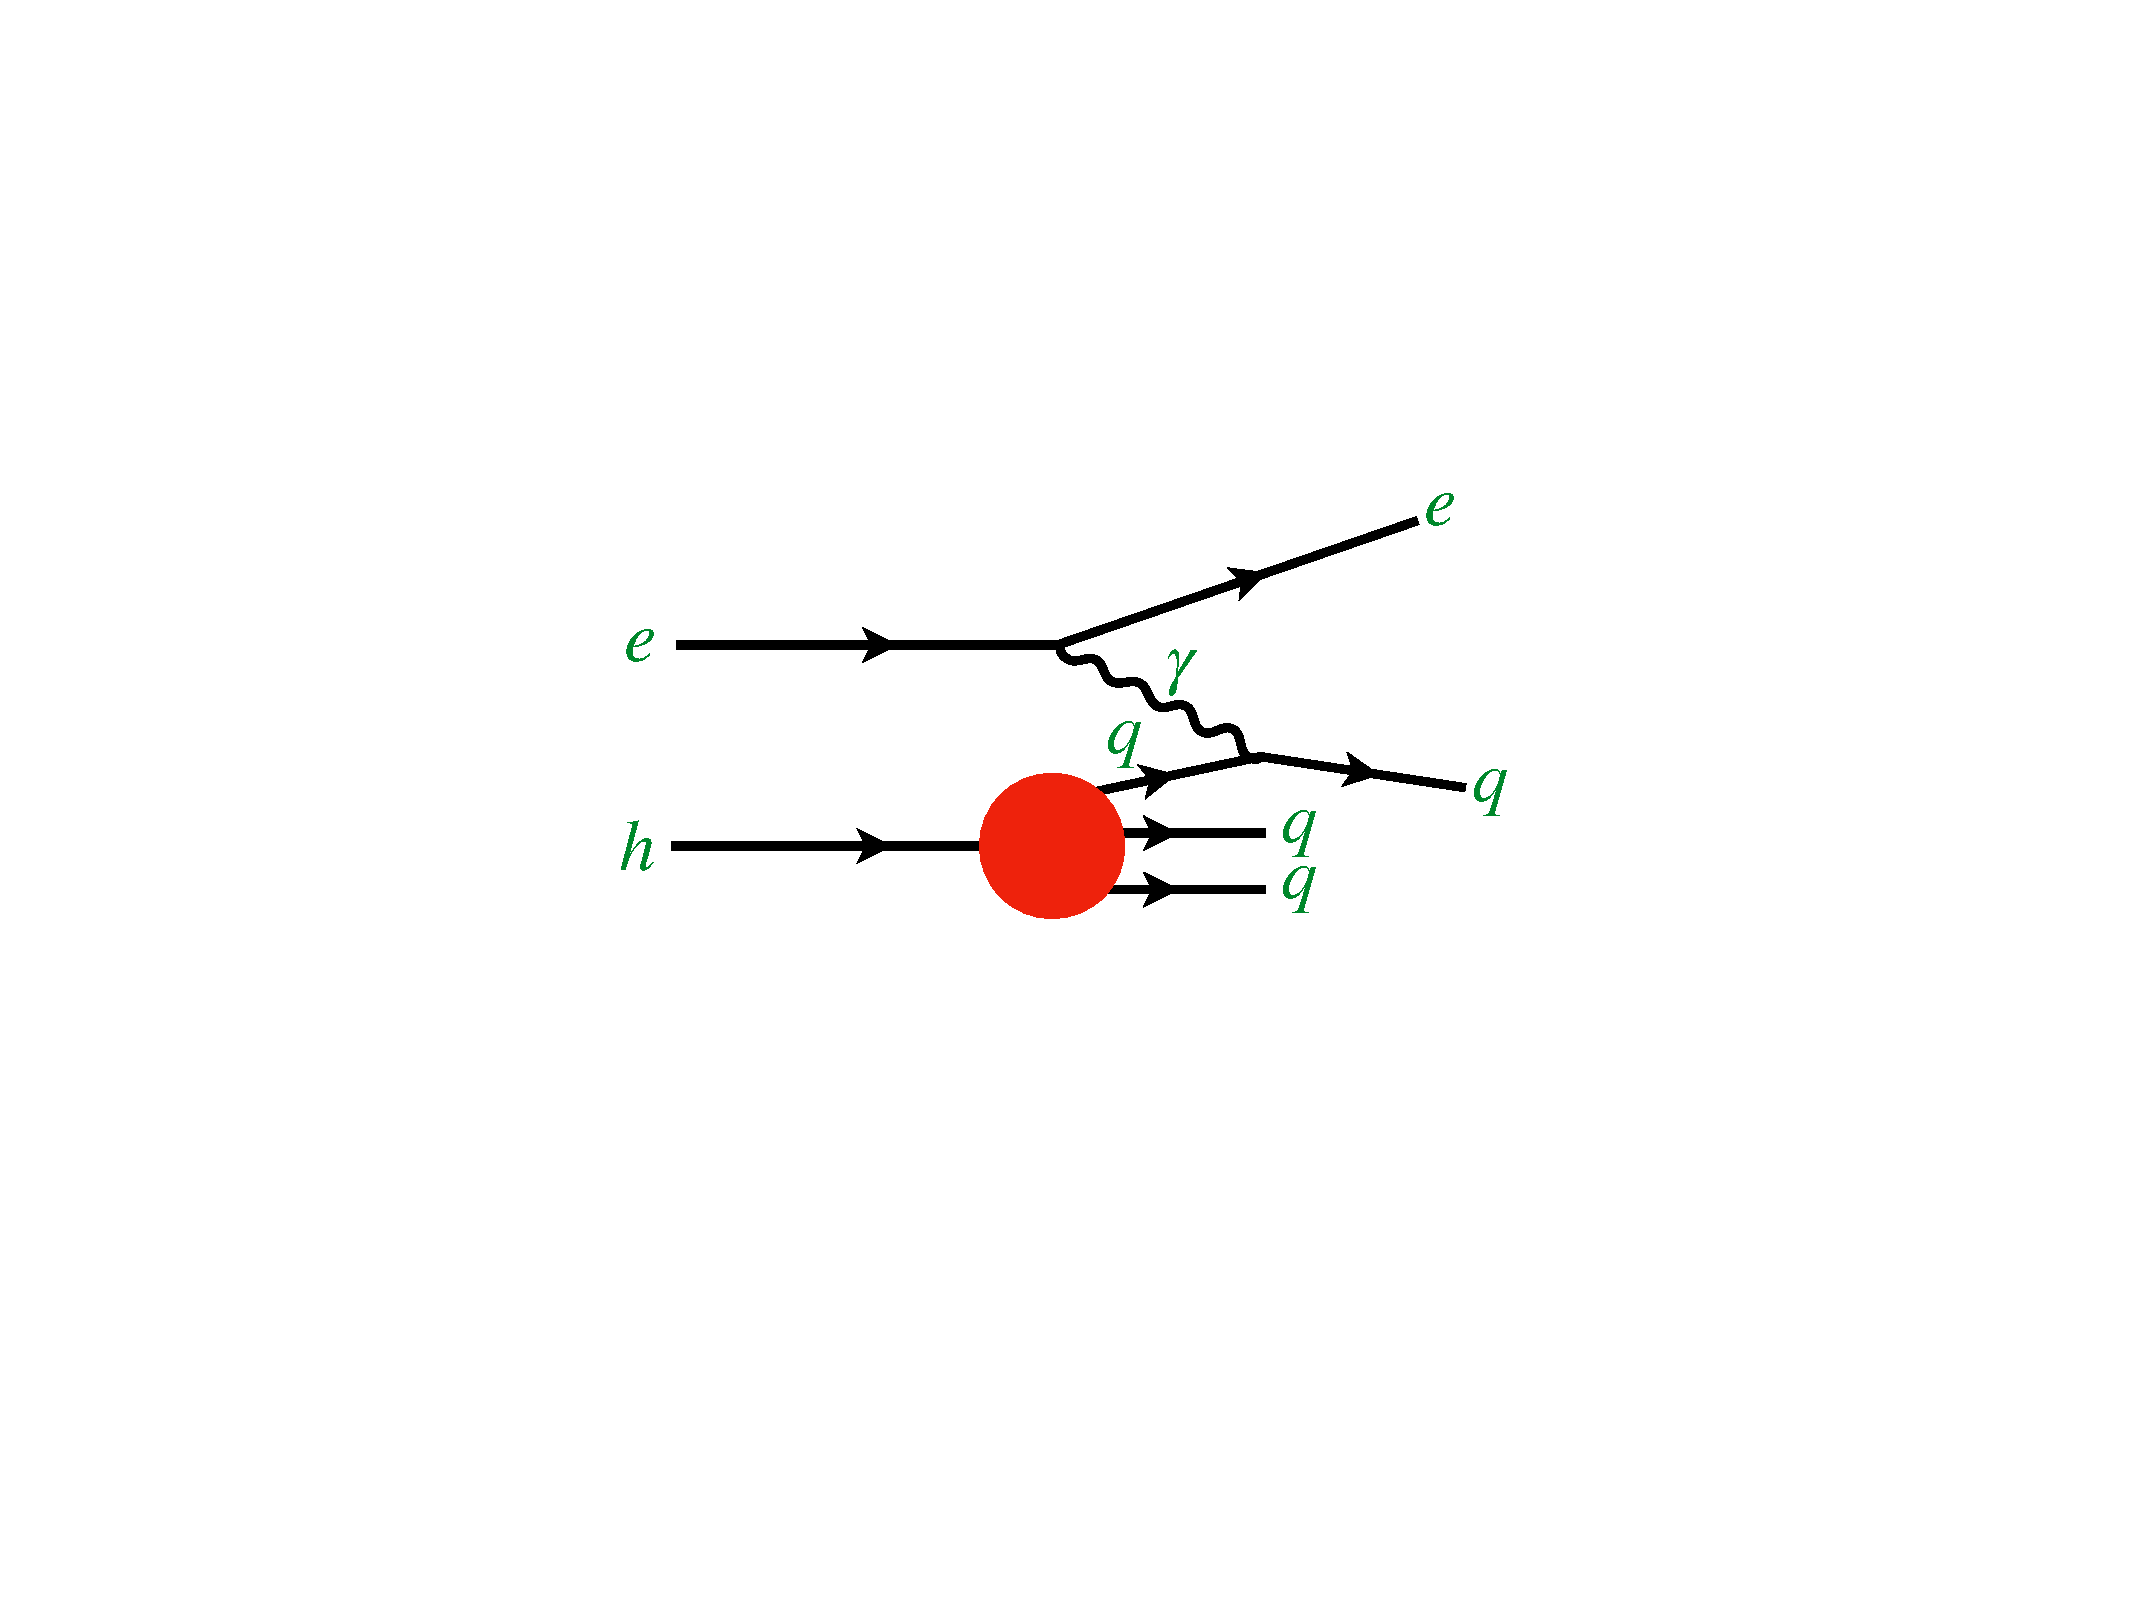
\includegraphics[width=0.35\textwidth]{figures/theory/DIS}
\caption{Schematic of the deep inelastic scattering experiment.}
\label{fig:dis_schematic}
\end{center}
\end{figure}


\subparagraph{Color Confinement}
The opposite end of the running coupling constant phenomenon is color confinement.
Proved to be a consequence of asymptotic freedom in Ref.~\cite{Nishijima1996}, this property of QCD described in Ref.~\cite{PhysRevD.10.2445} forbids the direct observation of free quarks and gluons, allowing only for composite particles that are color singlets.
While have been numerous efforts to understand the source of this phenomenon like in Refs.~\cite{BUCHMULLER1982479, KOGUT1976199, PhysRevD.31.2910, PhysRevD.57.2603, PhysRevD.62.114503, RevModPhys.55.775, PhysRevLett.90.102001}, these are based on numerical calculations.
An analytic proof of color confinement still escapes description and in fact, is one of the Millennium Problems \cite{MillenniumProb}.


%\subsection{Parton Distribution Functions}
%Deep ineslatic scattering experiments showed the internal point-like structure of a proton that can be described in terms of probability density functions called parton distribution functions.
%These are written in terms of the longitudinal momentum fraction carried by a constitutent proton, $x$, given as:
%
%\begin{align}
%x = \frac{Q^2}{2 P \dot q} = \frac{Q^2}{2 M \nu}
%\end{align}
%where $\nu$ is the energy of the photon shown in Figure~\ref{fig:dis_schematic}. This can be determined by 




%An analytic proof of the origin of color confinement is described in Ref.\cite{Gao:2018xsg}.
%==========================================================
%
%%QCD allows for predicting a variety of observables in particle reactions involving quarks and gluons in terms of the coupling constant $\alpha_s$.
%QCD amplitudes can be calculated by using the matrix elements for the basic diagrams shown in Figure~\ref{fig:qcd_diagrams} along with the quark and gluon propagators.Perturbative calculations done with the assumption that the coupling constant \alphas $ < 1 $ allow for 
%Another major feature 
% quark and gluon propagators along with teh corre
%
%
%

%The classical QCD Lagrangian is given by \cite{Chyla:2004zz}
%
%\begin{align}
%\mathcal{{L}}_{\mathrm{QCD}} = \sum_q \bar{\psi}_{q,a} (i \gamma^\mu \partial_\mu \delta_{ab} - g_s \gamma^\mu t_{ab}^C \mathcal{A}_\mu^C - m_q \delta_{ab}) \psi_{q,b} - \frac{1}{4} F_{\mu\nu}^A F^{A \mu\nu}
%\end{align}
%
%%\begin{align}
%%\mathcal{{L}}_{\mathrm{QCD}} &= \mathcal{L}_g + \mathcal{L}_q \\
%%&=  -\frac{1}{4} F_{\mu\nu} F^{\mu\nu} + \bar{\Psi}(i  \slashed{\partial} - m_q) \Psi + g \bar{\Psi} \gamma_\mu T \Psi A^\mu
%%\end{align}
%
%\begin{align}
%\mathcal{{L}}_{\mathrm{QCD}} =  -\frac{1}{4} F_{\mu\nu} F^{\mu\nu} + \bar{\Psi}(i  \slashed{\partial} - m_q) \Psi + g \bar{\Psi} \gamma_\mu T \Psi A^\mu
%\end{align}
%
%\begin{align}
%F^{\mu\nu}_a (x) \equiv \frac{\partial A_a^\nu (x)}{\partial x_\mu} - \frac{\partial A_a^\mu (x)}{\partial x_\nu}
%\end{align}
%
%%This Lagrangian is can be thought of as the sum of the quark and gluon terms $\mathcal{L}_g$ and $\mathcal{L}_q$, where
%%\begin{align}
%%\mathcal{L}_g &= - \frac{1}{4}\frac{1}{4} F_{\mu\nu} F^{\mu\nu} 
%%\end{align}
%
%
%where $Q$ is the momentum transfer in the particle reaction.This running coupling constant is small and asymptotically tends to zero at large energy scales (or at small distances) and is large at small energy scales (large distances).This can be seen in Figure \ref{fig:running_coupling}, which shows the $\alpha_s$ dependence on $Q$.This running coupling leads to two key behaviors discussed below.
%
%
%
%
